\smallframetitle

\section{From 17/06/24 to 21/06/24}
\insertsectionframe

\subsection{Road detection method - in progress}
\insertsubsectionframe

\begin{frame}{Methodology}
    We have seen that one classification with either DBScan or HDBScan isn't enough. So, why not combining them.
    \begin{block}{The base idea}
        We will combine the clusters of DBScan, HDBScan and OPTICS (another density base clustering method) to try to find roads.
    \end{block}

    \begin{block}{One problem}
        We are now able to detect road/railways but the problem is that there is still little clusters that are useless.
    \end{block}
\end{frame}

\begin{frame}{DBScan clustering}
    \begin{figure}
        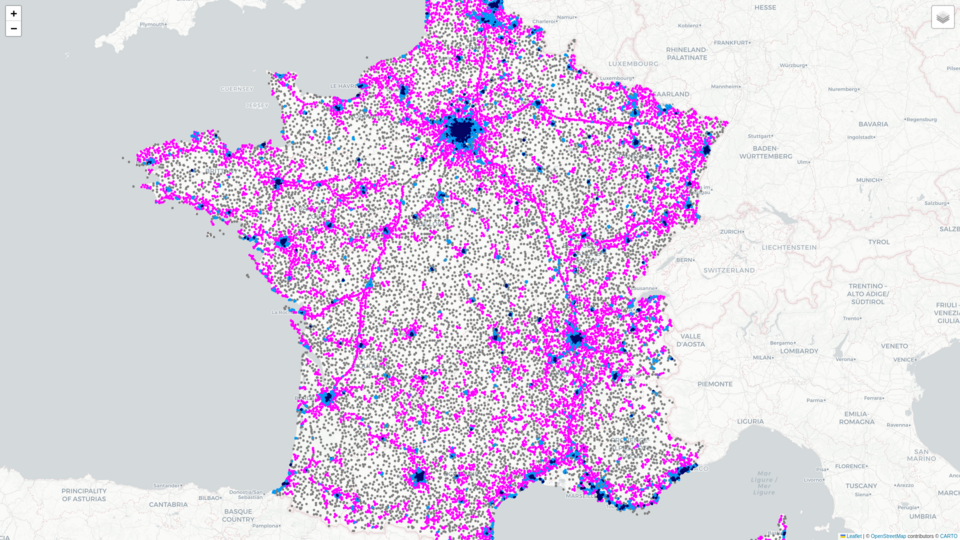
\includegraphics[height=0.6\paperheight]{images/cartes/road_detection/dbs.png}
        \caption{DBScan clustering}
    \end{figure}
\end{frame}

\begin{frame}{HDBScan clustering}
    \begin{figure}
        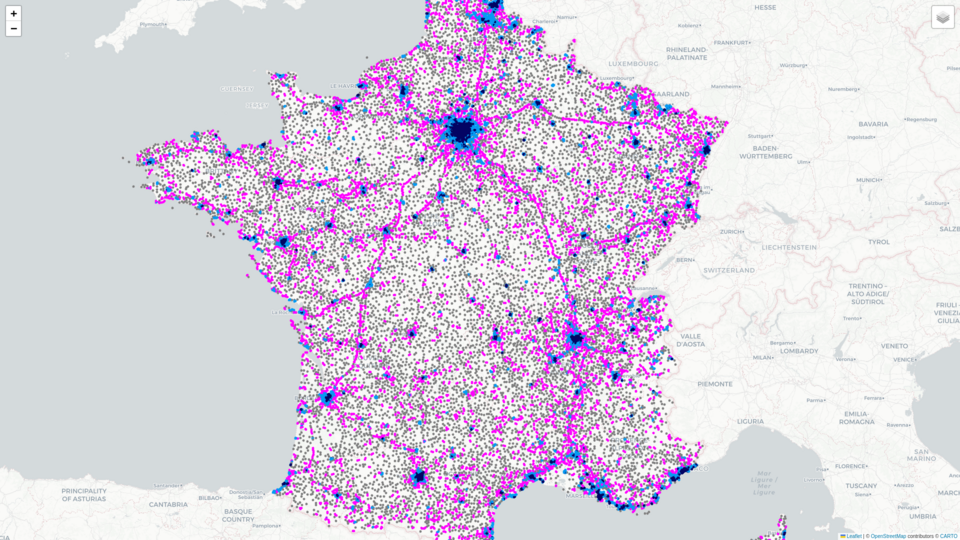
\includegraphics[height=0.6\paperheight]{images/cartes/road_detection/hdb.png}
        \caption{HDBScan clustering}
    \end{figure}
\end{frame}

\begin{frame}{OPTICS clustering}
    \begin{figure}
        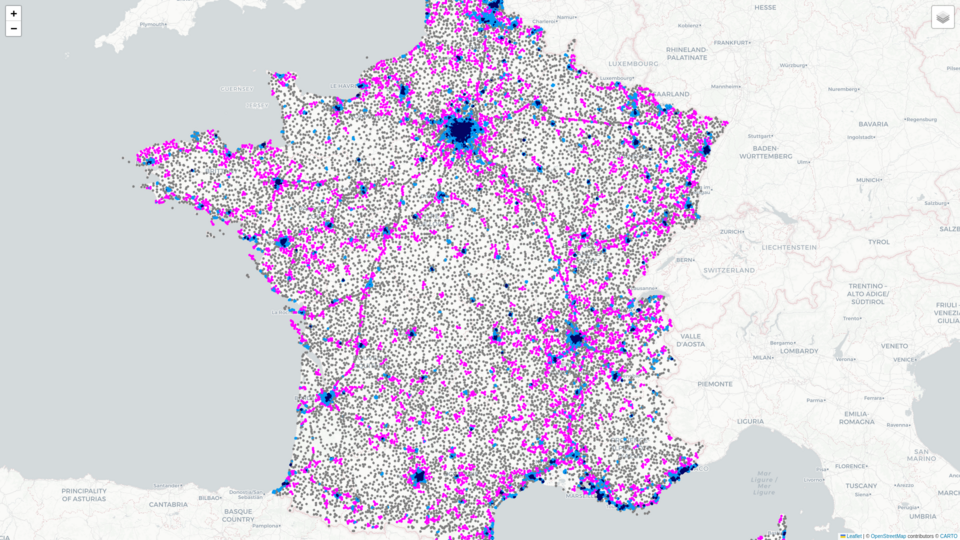
\includegraphics[height=0.6\paperheight]{images/cartes/road_detection/opt.png}
        \caption{OPTICS clustering}
    \end{figure}
\end{frame}

\begin{frame}{Result}
    \begin{figure}
        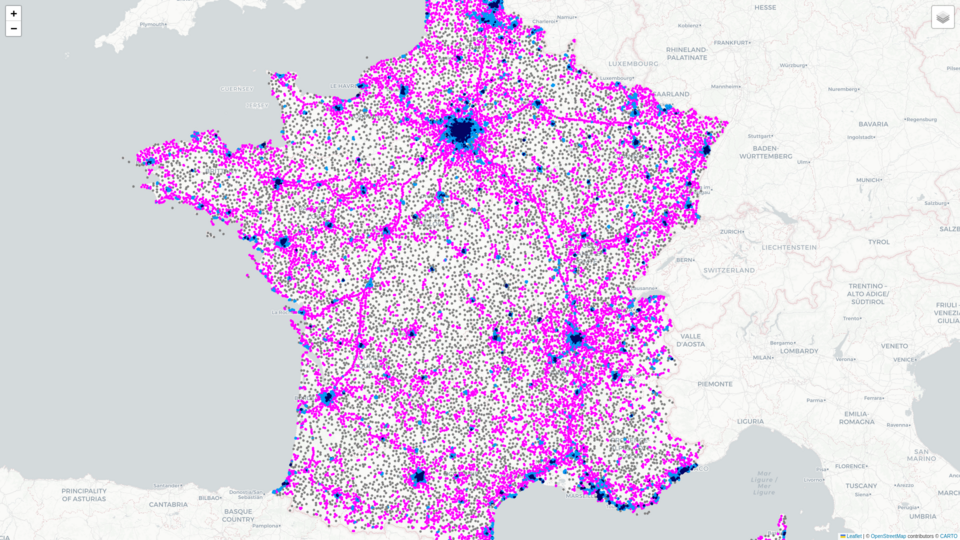
\includegraphics[height=0.6\paperheight]{images/cartes/road_detection/res.png}
        \caption{Road detection}
    \end{figure}
\end{frame}

\subsection{More details and problems}
\insertsubsectionframe

\begin{frame}{Detailed clusters detected}
    \begin{figure}
        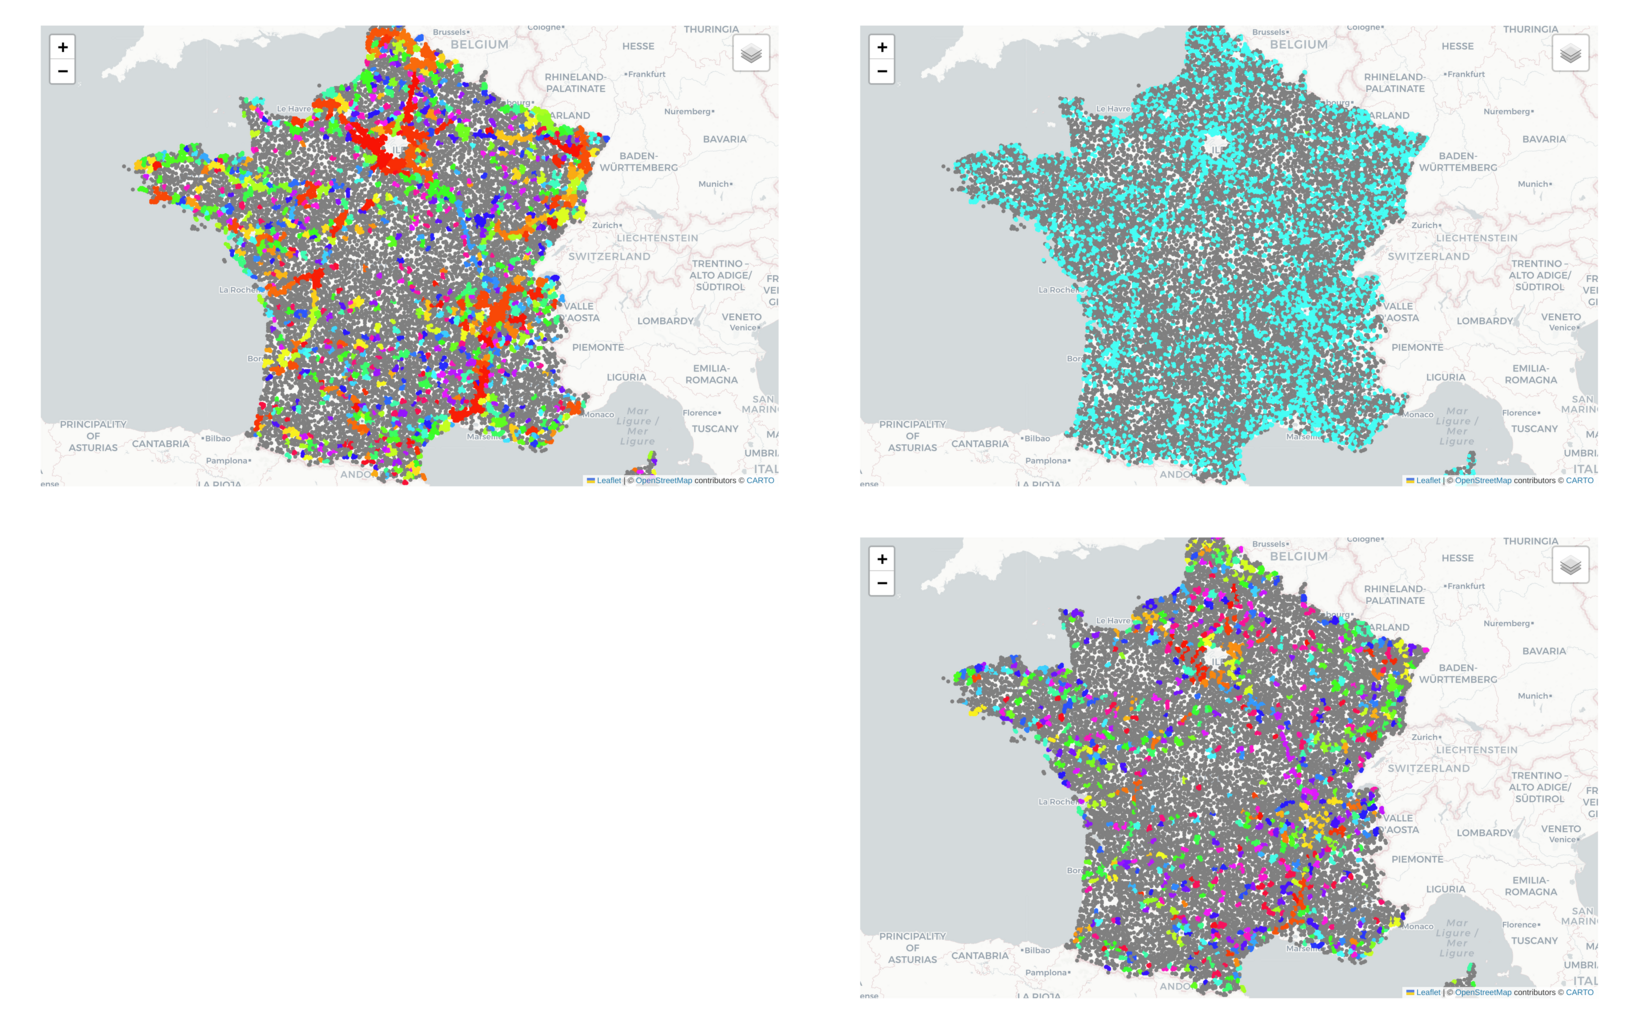
\includegraphics[height=0.6\paperheight]{images/clusters_road_detection.html.png}
        \caption{Detailed clusters detected in coutryside by each method}
    \end{figure}
\end{frame}

\begin{frame}{Problems and ideas}
    \begin{block}{Problems}
        \begin{itemize}
            \item A lot of little citys detected : not only roads ;
            \item The areas around big citys are a mess ;
            \item HDBScan has only one cluster.
        \end{itemize}
    \end{block}

    \begin{block}{Ideas}
        \begin{itemize}
            \item Refine the parameters of each method ;
            \item Use linear regressions to detect parts of roads and maybe help propagate them.
        \end{itemize}
    \end{block}
\end{frame}

\subsection{Modification of criteria}
\insertsubsectionframe

\begin{frame}{Altair AI Studio Software Review}
    Objective is to evaluate Altair AI Studio for their potential to enhance our research on classifying the terrain of mobile base stations.
    Available at: \url{https://altair.com/altair-ai-studio}
    \begin{block}{Altair AI Studio}
        This is a platform designed for data analysis and machine learning model building. Possible benefits for us:
        \begin{itemize}
            \item Simplifies data integration and visualization of base station and land cover data.
            \item Supports clustering and classification algorithms.
            \item Support for various machine learning algorithms.
            \item Enables effective result visualization (graphs) for enhanced analysis.
        \end{itemize}
    \end{block}
    \begin{columns}
        \begin{column}{0.4\paperwidth}
            \begin{block}{Key Features:}
                \begin{itemize}
                    \item Integration with various data sources.
                    \item Interactive model creation and testing.
                    \item Support for various machine learning algorithms.
                    \item User-friendly interface for data analysis and visualization.
                \end{itemize}
            \end{block}
        \end{column}
        \begin{column}{0.4\paperwidth}
            \begin{block}{Users:}
                \begin{itemize}
                    \item Data researchers
                    \item Analysts
                    \item Machine learning developers
                \end{itemize}
            \end{block}
        \end{column}
    \end{columns}
\end{frame}

\begin{frame}{Example of Usage in Altair AI Studio}
    \begin{figure}
        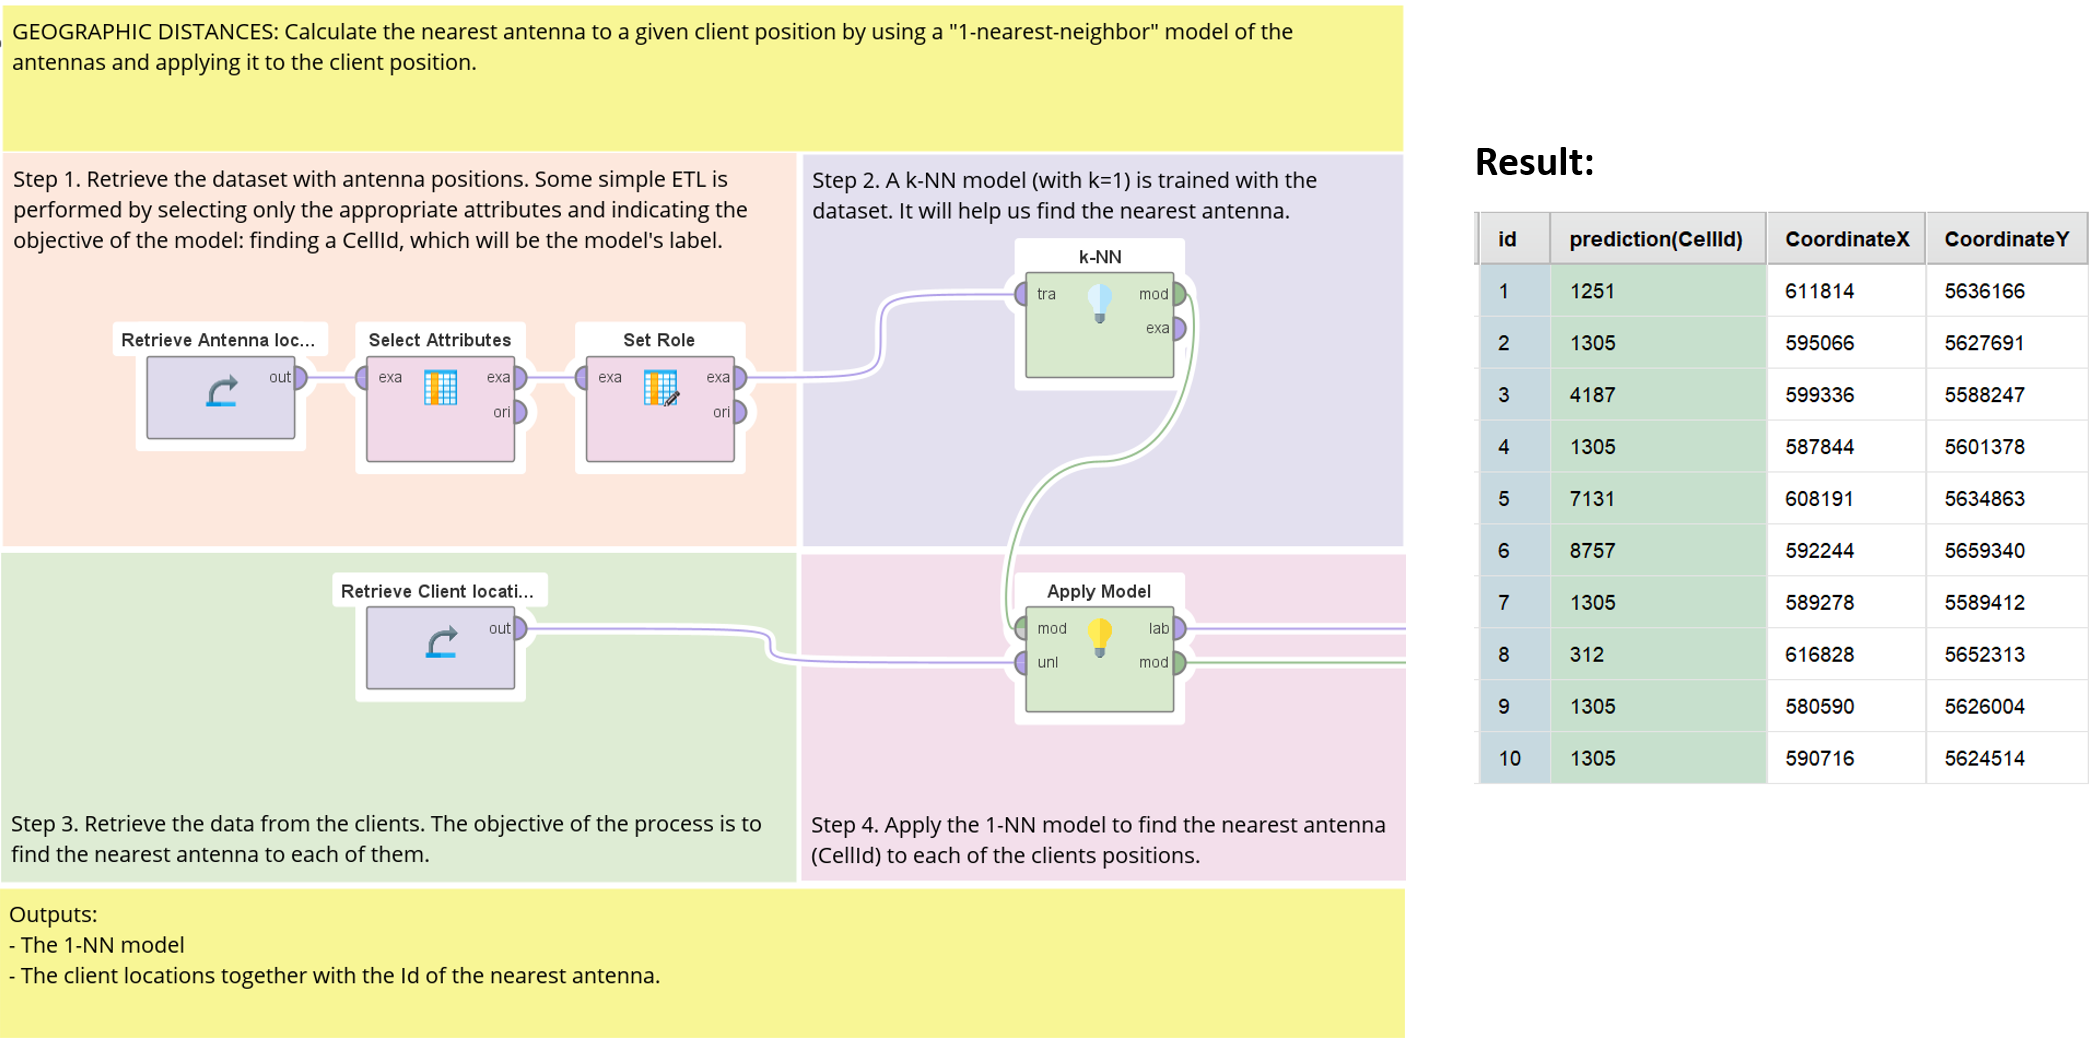
\includegraphics[height=0.6\paperheight]{images/Altair/Altair_proc_exmpl.png}
        \caption{How 3-NN method works}
    \end{figure}
\end{frame}
